\section{Theorie}


Relaxationserscheinungen werden beobachtet wenn ein System nicht-oszillatorisch
in seinen Ausgangszustand zurückkehrt, in dem Fall des RC-Kreises exponentiell.

Ein RC-Kreis besteht aus einem Wiederstand und einem Kondensator, die in Reihe
geschaltet sind. Wenn eine Spannungsquelle an diese Schaltung angeschlossen wird,
lädt sich der Kondensator auf. Für diesen Fall lässt sich eine Differentialgleichung
herleiten.

\begin{equation}
  \frac{dQ}{dt} = -\frac{1}{RC}\, Q(t)
\end{equation}

Mit den Anfangsbedingungen $Q(0)=0$ und $Q(\infty)= CU_0$ ergibt sich für den Aufladevorgang:

\begin{equation}
  Q(t) = CU_0 \left(1 - \exp\left(\frac{-t}{RC}\right)\right)
\end{equation}

Wenn die Spannungsquelle nach der Aufladung wieder entfernt, entlädt sich der Kondensator
wieder. Es ergibt sich für die Differentialgleichung die selbe wie beim Aufladevorgang,
nun sind allerdings die Anfangsbedingungen anders $Q(\infty) = 0$. Daraus ergibt sich dann
die Gleichung:

\begin{equation}
  Q(t) = Q(0)\, \exp\left(\frac{-t}{RC}\right)
  \label{eq:1}
\end{equation}

Die Zeitkonstante des Systems ist RC, denn sie beschreibt die Geschwindigkeit, mit
der sich das System seinen Endzustand annähert. Dabei ist R der Wiederstand des Wiederstandes
und C die Kapazität des Kondensators.\\\\

Für den Fall, dass die Spannungsquelle eine Sinusspannung mit der Frequenz $\omega$
ist, ergibt sich eine Phasenverschiebung $\phi(\omega)$ zwischen der Kondensatorspannung
und der Spannungsquelle. Diese Phasenverschiebung wird größer, je größer $\omega$ wird.

\begin{figure}
  \centering
  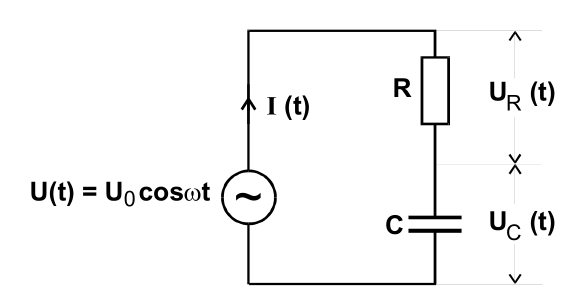
\includegraphics[height=5cm, width=0.7\textwidth]{Schaltungsbeispiel.png}
  \caption{Schaltungsbeispiel eines RC-Kreises mit Sinusspannung [1].}
\end{figure}

Um eine Gleichung für die Phasenverschiebung herzuleiten, wird zunächst die in Abbildung 1
gezeigte Schaltung mithilfe des Kirchhoffschen Gesetzes beschrieben.

\begin{equation}
  U(t) = U_R(t) + U_C(t)
\end{equation}

Damit ergibt sich die Gleichung:

\begin{equation}
  U_0 \cos(\omega t) = -A\omega RC \sin(\omega t + \phi) + \cos(\omega t + \phi)
\end{equation}

Wird der Fall $\omega t = \frac{\pi}{2}$ betrachtet folgt für die Phasenverschiebung:

\begin{equation}
  \phi(\omega) = \arctan(-\omega RC)
\end{equation}

Nun soll die Gleichung (5) für den Fall $\omega t + \phi = \frac{\pi}{2}$ betrachtet werden.
Damit lässt sich eine Gleichung für die Amplitude der Kondensatorspannung herleiten, die
auch von der Frequenz der Spannungsquelle abhängt.

\begin{equation}
  A(\omega) = \frac{U_0}{\sqrt{1+\omega^2 R^2 C^2}}
\end{equation}

Die Gleichung (4) wird nun mit der Relation $I(t) = C\frac{dU_C}{dt}$ umgeschrieben zu:\\\\

$U(t) = RC \frac{dU_C}{dt} + U_C(t)$\\\\

Unter der Vorraussetzung, dass $\omega >> \frac{1}{RC}$ ist kann die Gleichung
zu einem Integral umgeformt werden:

\begin{equation}
  U_C(t) = \frac{1}{RC} \int_{0}^{t} U(t')  \, \symup{d}t'
\end{equation}
